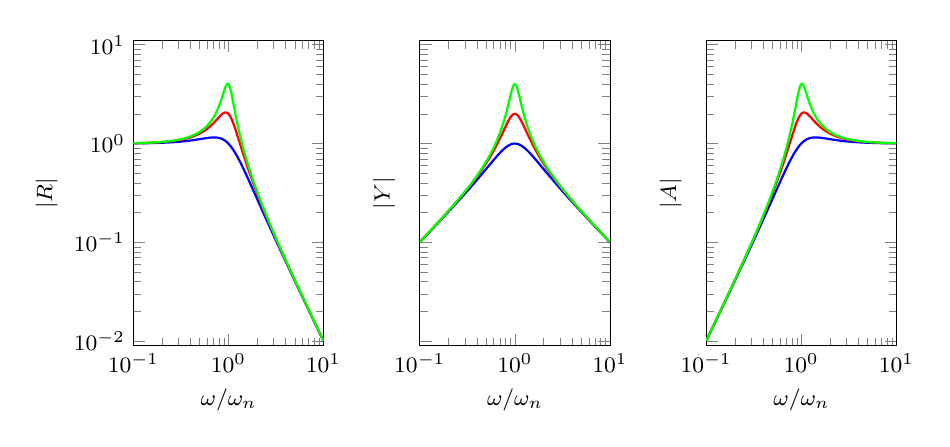
\begin{tikzpicture}[scale=1]
	\footnotesize
	\begin{axis}[
		at={(0,0)},
		width=0.33\textwidth,
		height=0.45\textwidth,
		xlabel={$\omega/\omega_n$},
		ylabel = {$|R|$},
		xmax=10.1,
		xmin=0.1,
		ymax=11,
		ymin=0.009 ,
		samples=1000,
		xmode=log,
		ymode=log,
		ylabel near ticks]
		
		
		\def\k{1};
		\def\zetaB{0.5};
		\def\zetaC{0.25};
		\def\zetaD{0.125};		

		
		\addplot[blue, thick, domain=0.1:10] (x, {1/sqrt(\k^2*(1-(x)^2)^2 + (\zetaB*2*\k*(x))^2)});		
		\addplot[red, thick, domain=0.1:10] (x, {1/sqrt(\k^2*(1-(x)^2)^2 + (\zetaC*2*\k*(x))^2)});		
		\addplot[green, thick, domain=0.1:10] (x, {1/sqrt(\k^2*(1-(x)^2)^2 + (\zetaD*2*\k*(x))^2)});		
		
%		\draw [thick, dashed] (axis cs: 1, 0.001) -- (axis cs: 1,11);

	\end{axis}

	\begin{axis}[
	at={(0.3\textwidth,0)},
	width=0.33\textwidth,
	height=0.45\textwidth,
	xlabel={$\omega/\omega_n$},
	ylabel = {$|Y|$},
	yticklabel=\empty,
	xmax=10.1,
	xmin=0.1,
	ymax=11,
	ymin=0.009 ,
	samples=1000,
	xmode=log,
	ymode=log,
	ylabel near ticks]
	
	
	\def\k{1};
	\def\zetaB{0.5};
	\def\zetaC{0.25};
	\def\zetaD{0.125};		
	
	
	\addplot[blue, thick, domain=0.1:10] (x, {x/sqrt(\k^2*(1-(x)^2)^2 + (\zetaB*2*\k*(x))^2)});		
	\addplot[red, thick, domain=0.1:10] (x, {x/sqrt(\k^2*(1-(x)^2)^2 + (\zetaC*2*\k*(x))^2)});		
	\addplot[green, thick, domain=0.1:10] (x, {x/sqrt(\k^2*(1-(x)^2)^2 + (\zetaD*2*\k*(x))^2)});		
	
	%		\draw [thick, dashed] (axis cs: 1, 0.001) -- (axis cs: 1,11);
	
\end{axis}

	\begin{axis}[
	at={(0.6\textwidth,0)},
	width=0.33\textwidth,
	height=0.45\textwidth,
	xlabel={$\omega/\omega_n$},
		ylabel = {$|A|$},
	yticklabel=\empty,
	xmax=10.1,
	xmin=0.1,
	ymax=11,
	ymin=0.009 ,
	samples=1000,
	xmode=log,
	ymode=log,
	ylabel near ticks]
	
	
	\def\k{1};
	\def\zetaB{0.5};
	\def\zetaC{0.25};
	\def\zetaD{0.125};		
	
	
	\addplot[blue, thick, domain=0.1:10] (x, {x^2/sqrt(\k^2*(1-(x)^2)^2 + (\zetaB*2*\k*(x))^2)});		
	\addplot[red, thick, domain=0.1:10] (x, {x^2/sqrt(\k^2*(1-(x)^2)^2 + (\zetaC*2*\k*(x))^2)});		
	\addplot[green, thick, domain=0.1:10] (x, {x^2/sqrt(\k^2*(1-(x)^2)^2 + (\zetaD*2*\k*(x))^2)});		
	
	%		\draw [thick, dashed] (axis cs: 1, 0.001) -- (axis cs: 1,11);
	
\end{axis}
	
\end{tikzpicture}